\documentclass[12pt]{article}
\usepackage{fancyvrb,amsmath,amsfonts,amssymb,graphicx,listings}
\usepackage[usenames,dvipsnames,svgnames,table]{xcolor}
%\usepackage{parskip}
\usepackage{slashed}
\usepackage{tikz}
\usepackage{mathrsfs}

% change margins
\addtolength{\oddsidemargin}{-.875in}
\addtolength{\evensidemargin}{-.875in}
\addtolength{\textwidth}{1.75in}
\addtolength{\topmargin}{-.875in}
\addtolength{\textheight}{1.75in}

\hyphenpenalty=10000

\begin{document}

\begin{center}
{\sc rutherford scattering}
\end{center}

\noindent
Consider an electron scattered by an atomic nucleus.\footnote{
The original Rutherford scattering experiment in 1911 used alpha particles, not electrons.
However, scattering of any charged particle by Coulomb interaction
is now known as Rutherford scattering.
The first Rutherford scattering experiment using electrons appears to have
been done by F.~L.~Arnot, then a student of Rutherford, in 1929.}
\begin{center}
\begin{tikzpicture}
\draw[dashed] (0,0) circle (0.5cm);
%\draw[dashed] (1.4,0) -- (0.6,0);
\draw[thick,->] (-2,0) node[anchor=east] {$e^-$} -- (-0.6,0);
\draw[thick,->] (0.40,0.40) -- (1.3,1.3) node[anchor=south west] {$e^-$};
\draw (1,0.5) node {$\theta$};
\end{tikzpicture}
\end{center}

\noindent
Here is the same diagram with momentum and spinor labels.
\begin{center}
\begin{tikzpicture}
\draw[dashed] (0,0) circle (0.5cm);
%\draw[dashed] (1.4,0) -- (0.6,0);
\draw[thick,->] (-2,0) node[anchor=east] {$p_1,u_1$} -- (-0.6,0);
\draw[thick,->] (0.40,0.40) -- (1.3,1.3) node[anchor=south west] {$p_2,u_2$};
\draw (1,0.5) node {$\theta$};
\end{tikzpicture}
\end{center}

\noindent
For a typical scattering experiment the momentum vectors are
$$
p_1=\begin{pmatrix}E\\0\\0\\p\end{pmatrix}\qquad
p_2=\begin{pmatrix}
E\\
p\sin\theta\cos\phi\\
p\sin\theta\sin\phi\\
p\cos\theta
\end{pmatrix}
$$

\noindent
where $E=\sqrt{p^2+m^2}$.
Symbol $p$ is electron momentum and $m$ is electron mass.
The spinors are
\begin{align*}
u_{11}=\begin{pmatrix}E+m\\0\\p\\0\end{pmatrix}
\qquad
u_{21}=\begin{pmatrix}E+m\\0\\p_2^z\\p_2^x+ip_2^y\end{pmatrix}
\\
u_{12}=\begin{pmatrix}0\\E+m\\0\\-p\end{pmatrix}
\qquad
u_{22}=\begin{pmatrix}0\\E+m\\p_2^x-ip_2^y\\-p_2^z\end{pmatrix}
\end{align*}

\noindent
The second digit in a spinor subscript is the spin state.
The spinors are not normalized.
Instead, a combined spinor normalization constant $N=(E+m)^2$ is used.

\bigskip
\noindent
The probability density for Rutherford scattering is
\begin{equation*}
|\mathcal{M}(s_1,s_2)|^2=\frac{Z^2e^4}{q^4}\frac{1}{N}\left|\bar{u}_2\gamma^0 u_1\right|^2
\end{equation*}

\noindent
Symbol $s_j$ selects the spin of spinor $j$,
$Z$ is the atomic number of the nucleus,
$e$ is electron charge,
and $q$ is momentum transfer $q=p_1-p_2$, $q^4=16p^4\sin^4(\theta/2)$.

\bigskip
\noindent
The expected probability density
$\langle\vert\mathcal{M}\vert^2\rangle$
is computed by summing $|\mathcal{M}|^2$
over all four spin states and then dividing by the number of inbound states.
There are two inbound states.
\begin{align*}
\langle\vert\mathcal{M}\vert^2\rangle
&=\frac{1}{2}\sum_{s_1=1}^2\sum_{s_2=1}^2\left|\mathcal{M}(s_1,s_2)\right|^2
\\
&=\frac{Z^2e^4}{2q^4}\frac{1}{N}\sum_{s_1=1}^2\sum_{s_2=1}^2\left|\bar{u}_2\gamma^0 u_1\right|^2
\\
&=\frac{Z^2e^4}{2q^4}\mathop{\rm Tr}\left((\slashed{p}_1+m)\gamma^0(\slashed{p}_2+m)\gamma^0\right)
\\
&=\frac{2Z^2e^4}{q^4}\left(E^2+m^2+p^2\cos\theta\right)
\end{align*}

\noindent
Run ``rutherford-scattering-1.txt'' to verify that
$$
\frac{1}{N}\sum_{s_1=1}^2\sum_{s_2=1}^2\left|\bar{u}_2\gamma^0 u_1\right|^2
=\mathop{\rm Tr}\left((\slashed{p}_1+m)\gamma^0(\slashed{p}_2+m)\gamma^0\right)
$$

\noindent
Run ``rutherford-scattering-2.txt'' to verify that
$$
\frac{1}{2}
\mathop{\rm Tr}\left((\slashed{p}_1+m)\gamma^0(\slashed{p}_2+m)\gamma^0\right)
=2(E^2+m^2+p^2\cos\theta)
$$

\noindent
and
\begin{equation*}
(p_1-p_2)^4=16p^4\sin^4(\theta/2)
\end{equation*}

\noindent
For low energy electron beams such that $p\ll m$ we have
\begin{equation*}
E^2+m^2+p^2\cos\theta\approx2m^2
\end{equation*}

\noindent
Hence
\begin{equation*}
\langle|\mathcal{M}|^2\rangle=\frac{Z^2e^4m^2}{4p^4\sin^4(\theta/2)}
\end{equation*}

\noindent
The differential cross section is
\begin{equation*}
\frac{d\sigma}{d\Omega}=\frac{\langle|\mathcal{M}|^2\rangle}{16\pi^2}
\end{equation*}

\noindent
From $e^2=4\pi\alpha$ and $(\cos\theta-1)^2=4\sin^4(\theta/2)$ we have
\begin{equation*}
\frac{d\sigma}{d\Omega}
=\frac{Z^2\alpha^2m^2}{p^4(\cos\theta-1)^2}
\end{equation*}

\newpage
\noindent
We can integrate $d\sigma$ to obtain a cumulative distribution function.

\bigskip
\noindent
Let
\begin{equation*}
I(\theta)=\int_\alpha^\xi\frac{d\sigma}{d\Omega}\,\sin\theta\,d\theta,
\quad\alpha\le\xi\le\pi
\end{equation*}

\noindent
for some $\alpha>0$.
The support interval is restricted because $d\sigma$ is undefined for $\theta=0$.

\bigskip
\noindent
The cumulative distribution function is
\begin{equation*}
F(\theta)=\frac{I(\theta)}{I(\pi)},
\quad\alpha\le\theta\le\pi
\end{equation*}

\noindent
Hence
\begin{equation*}
P(\theta_1\le\theta\le\theta_2)=F(\theta_2)-F(\theta_1)
\end{equation*}

\noindent
The probability density is
\begin{equation*}
f(\theta)=\frac{dF(\theta)}{d\theta}=\frac{1}{I(\pi)}\frac{d\sigma}{d\Omega}\sin\theta,
\qquad\alpha\le\theta\le\pi
\end{equation*}

\noindent
Run ``rutherford-scattering-3.txt'' to draw a graph of $f(\theta)$ for $\alpha=\tfrac{1}{4}\pi=45^\circ$.

\begin{center}
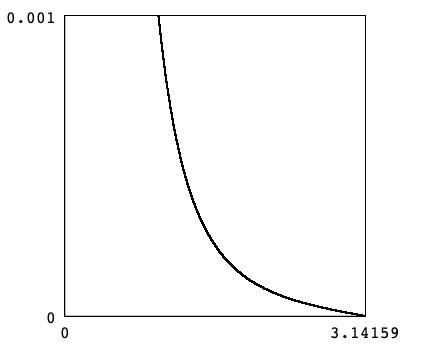
\includegraphics[scale=0.5]{rutherford-scattering-ss1.png}
\end{center}

\noindent
The following table shows the corresponding probability distribution for three bins.

\begin{center}
\begin{tabular}{|c|c|c|}
\hline
$\theta_1$ & $\theta_2$ & $P(\theta_1\le\theta\le\theta_2)$\\
\hline
$0^\circ$ & $45^\circ$ & -- \\
$45^\circ$ & $90^\circ$ & 0.83 \\
$90^\circ$ & $135^\circ$ & 0.14 \\
$135^\circ$ & $180^\circ$ & 0.03 \\
\hline
\end{tabular}
\end{center}

\end{document}
